%%%%%%%%%%%%%%%%%%%%%%%%%%%%%%%%
% Section 5 in the alt (empirical-first) ordering.
% RSP definition and branching-event/state terminology are introduced in
% §3.1; this section explains the mechanism behind the empirical patterns
% of §3-§4 along a single quantity --- the attention mass scalar w.
%%%%%%%%%%%%%%%%%%%%%%%%%%%%%%%%

\section{Why RSP Works}\label{sec:why_rsp_works}

Sections~\ref{sec:experimental_analysis} and~\ref{sec:application} documented four empirical patterns RSP induces: early-stage entropy rise, trajectory-level diversification, Pass@$N$ accumulation under independent draws, and a late-training advantage in DAPO. We now explain these patterns mechanistically. RSP does not add to the hidden state directly but enters only through attention weights, so within one attention head its instantaneous influence reduces to a single scalar: the \emph{attention mass} $w$ on RSP tokens. This section tracks how that scalar evolves. Early on, $w$ is large enough to branch the hidden state into multiple directions (\S\ref{sec:improve}); as the KV cache grows, its upper bound narrows and the response converges (\S\ref{sec:converge}). Randomness supplies \emph{independent} perturbations across rollouts so that each opens a fresh branch. We assume the RSP definition and the \emph{branching event/state} terminology of \S\ref{sec:rsp_definition}; further proofs are in Appendix~\ref{app:proofs}.

% ================================================================
\subsection{Exploration: RSP strengthens early-stage exploration}\label{sec:improve}\label{sec:multipath}
% ================================================================

Inserting a random prompt concentrates attention on it, and that concentration is what amplifies exploration. The effect of a single RSP injection on the hidden state can be examined along two questions: \emph{how much}, and \emph{in which direction}. The first is decided by a single scalar $w$ inside one attention head, the second by the distribution of $\mathbf{H}$. RSP's design choice, an isotropic Gaussian, addresses both at once.

Consider one attention head in self-attention layer $\ell$. At query position $i$, the query attends $n\ge1$ unmasked real tokens together with $L\ge1$ RSP tokens, all attention logits finite. Write the attention weights as $\alpha_{ij}^{(\ell)}$ and the value vectors on the real and RSP sides as $\mathbf{v}_j^{(\ell)},\mathbf{v}_{r_j}^{(\ell)}$. Defining the total attention mass on random tokens $w_{r,i}^{(\ell)} := \sum_{j=1}^L \alpha_{i,n+j}^{(\ell)}$, the real-token mass $1-w_{r,i}^{(\ell)}$ is positive and the head output $\mathbf{o}_i^{(\ell)}$ splits \emph{exactly} into a renormalized real-token term $\tilde{\mathbf{o}}_i^{(\ell)}$ and an RSP-induced contribution $\boldsymbol{\eta}_i^{(\ell)}$:
\begin{equation}\label{eq:decomp}
\mathbf{o}_i^{(\ell)}
\;=\;
(1-w_{r,i}^{(\ell)})\,\tilde{\mathbf{o}}_i^{(\ell)}
\;+\;
\boldsymbol{\eta}_i^{(\ell)},
\quad
\tilde{\mathbf{o}}_i^{(\ell)} := \sum_{j=1}^n \tfrac{\alpha_{ij}^{(\ell)}}{1-w_{r,i}^{(\ell)}}\,\mathbf{v}_j^{(\ell)},
\quad
\boldsymbol{\eta}_i^{(\ell)} := \sum_{j=1}^L \alpha_{i,n+j}^{(\ell)}\mathbf{v}_{r_j}^{(\ell)}.
\end{equation}

\begin{proof}[Derivation of Eq.~\eqref{eq:decomp}]
Write the head output as $\sum_{j=1}^{n}\alpha_{ij}^{(\ell)}\mathbf{v}_{j}^{(\ell)}+\sum_{j=1}^{L}\alpha_{i,n+j}^{(\ell)}\mathbf{v}_{r_j}^{(\ell)}$, then factor $1-w_{r,i}^{(\ell)} = \sum_{j=1}^n \alpha_{ij}^{(\ell)}>0$ out of the real-token sum. No approximation beyond the softmax-normalization identity is used.
\end{proof}

This single quantity $w_{r,i}^{(\ell)}$ controls both the attenuation ratio $1-w_{r,i}^{(\ell)}$ on the real signal and the upper bound on the random contribution $\|\boldsymbol{\eta}_i^{(\ell)}\| \le w_{r,i}^{(\ell)}\,\max_j \|\mathbf{v}_{r_j}^{(\ell)}\|$. The \emph{magnitude} of RSP-induced variation thus reduces to one number in $[0,1]$. Early in decoding the KV cache is short and this value is non-negligible, so a single RSP draw can perturb next-token decisions.

The scalar $w$ alone, however, controls only \emph{how much} and not \emph{where} the perturbation lands; the direction is decided by the distribution of $\mathbf{H}$. The transformer's logit map is non-linear in its inputs, but a first-order Taylor expansion around the linearization point $\bar h = 0$ gives the local surrogate $\Delta_{ij}(\bar h) \approx \Delta_{ij}(0) + b_{ij}^\top \bar h$, where $z_i$ is the logit at vocab token $i$, $\Delta_{ij} := z_i - z_j$, and $b_{ij} := \nabla_{\bar h}(\Delta_{ij})|_{\bar h=0}$ is the gradient direction along which tokens $i$ and $j$ swap rank (in general $b_{ij}$ is not unit-norm). Since RSP is training-free, we cannot know in advance which $b_{ij}$ opens a useful branch on a given problem, and this missing prior constrains the distribution design. A deterministic injected sequence pins its contribution to a single direction and leaves the orthogonal complement unperturbed. Uniform sampling from the vocabulary is random but inherits the anisotropic geometry of the token-embedding table, so some directions remain systematically under-perturbed. With no prior to lean on, the prudent design is to maximize the worst-case directional variance under a fixed variance budget; that solution is uniquely isotropic.

\begin{proposition}[Maximin directional coverage]\label{thm:minimax_directional_coverage}
Let $D$ be any zero-mean distribution on $\mathbb{R}^d$ with covariance $\Sigma_D$ and trace budget $\mathrm{tr}(\Sigma_D)\le\rho^2$. Then $\min_{\|b\|=1}\mathrm{Var}_{h\sim D}(b^\top h) = \lambda_{\min}(\Sigma_D) \le \rho^2/d$, with equality if and only if $\Sigma_D = (\rho^2/d)\mathbf{I}_d$.
\end{proposition}

This is a \emph{design criterion} for the prompt law, not a guarantee of correctness; correctness enters through the task-side $p_{\min}(x)$ assumption of \S\ref{sec:converge} and independent resampling.\footnote{The maximin is stated in input space; isotropy is not claimed to be preserved through the transformer. Any local logit direction pulls back via the model Jacobian to an input-space direction $b$, and isotropy guarantees only that no such pulled-back direction has zero projected variance.}

Gaussian RSP satisfies the equality with $\Sigma = \sigma_E^2 \mathbf{I}_d$ and adds \emph{full support} on $\mathbb{R}^d$ (Appendix~\ref{app:why_random}). The two roles separate cleanly. Isotropy ensures no direction is systematically excluded. Full support, in turn, gives positive probability to the open branching-event region (\S\ref{sec:rsp_definition}) whenever it is non-empty (Appendix~\ref{app:topk_entry}). Monotone temperature preserves ranking and cannot reach this region, so RSP's \emph{rank-changing} branching follows from the two properties together. This is the mechanism that splits the hidden state into multiple branching states early in reasoning.

% ================================================================
\subsection{Annealing: KV cache growth dilutes RSP attention}\label{sec:converge}
% ================================================================

The early branching that RSP introduces stabilizes naturally as decoding proceeds: the upper bound on the same scalar $w_{r,i}^{(\ell)}$ defined in \S\ref{sec:improve} narrows along the sequence axis with autoregressive KV cache growth. Each step appends one real-token term while the number of RSP terms is fixed; freezing the logit gap between real and RSP tokens, this asymmetry yields the following exact bound.

\begin{theorem}[Attention-mass decay under KV cache growth]\label{thm:decay}
Consider a single attention head with per-head key dimension $d_{\text{head}}$, where query $\mathbf{q}_i$ at position $i$ attends $n\ge1$ real keys $\mathbf{k}_j$ and $L\ge1$ RSP keys $\mathbf{k}_{r_{j'}}$ under finite logits. Define the pre-scale logit gap $\Delta_i := \min_{j\in[n]}\mathbf{q}_i^\top\mathbf{k}_j - \max_{j'\in[L]}\mathbf{q}_i^\top\mathbf{k}_{r_{j'}}$. In scaled dot-product attention,
\[
w_{r,i} \;\le\; \frac{L}{L + n\,\exp(\Delta_i/\sqrt{d_{\text{head}}})},
\]
and the right-hand side is strictly decreasing in $n$ and tends to $0$ at fixed $L$ and $\Delta_i$.
\end{theorem}

\begin{proof}
Let $s_j := \mathbf{q}_i^\top\mathbf{k}_j/\sqrt{d_{\text{head}}}$, $s_{r_{j'}} := \mathbf{q}_i^\top\mathbf{k}_{r_{j'}}/\sqrt{d_{\text{head}}}$, $s_{r,\max} := \max_{j'} s_{r_{j'}}$, and $R := \sum_{j'=1}^L \exp(s_{r_{j'}})$. The gap definition gives $s_j \ge \Delta_i/\sqrt{d_{\text{head}}} + s_{r,\max}$ for every real $j$, and $\exp(s_{r,\max}) \ge R/L$ holds because the max dominates the average; combining the two and summing over the $n$ real keys yields $\sum_{j=1}^n \exp(s_j) \ge (n/L)\exp(\Delta_i/\sqrt{d_{\text{head}}})\,R$. Substituting into $w_{r,i} = R/(\sum_j\exp(s_j) + R)$ gives
\[
w_{r,i}
\;\le\;
\frac{R}{(n/L)\exp(\Delta_i/\sqrt{d_{\text{head}}})\,R + R}
\;=\;
\frac{L}{L + n\,\exp(\Delta_i/\sqrt{d_{\text{head}}})}.
\]
The derivative of the right-hand side in $n$ is $-L\exp(\Delta_i/\sqrt{d_{\text{head}}})/(L + n\exp(\Delta_i/\sqrt{d_{\text{head}}}))^2 < 0$, so the bound is strictly decreasing and tends to $0$ as $n\to\infty$.
\end{proof}

Applied at each layer $\ell$ to the scalar $w_{r,i}^{(\ell)}$ of \S\ref{sec:improve}: $L$ caps maximum influence while $n$ grows automatically each step, narrowing the upper bound. The theorem guarantees only sequence-axis attenuation at a fixed (layer, query, gap); it does not assert layer-axis monotone decay. The gap does evolve during decoding but tends to sharpen at deeper layers and longer sequences, with Figure~\ref{fig:attention_mass}(a)'s layer-axis attenuation as indirect evidence. The accurate reading is therefore ``the attainable upper bound at a fixed gap decreases monotonically,'' not ``realized mass decreases per step.'' Since Eq.~\eqref{eq:decomp} ties the random contribution to the same scalar, branching-event reachability (\S\ref{sec:rsp_definition}) inherits the envelope: as the cache grows, new branching events become rarer and the response commits to the branch already opened, yielding an implicit explore-then-exploit. Figure~\ref{fig:attention_mass} confirms how this envelope manifests in the actual model: the sequence-axis decrease matches Theorem~\ref{thm:decay}'s prediction directly, and the additional layer-axis attenuation is observed empirically and lies outside the theorem's scope.

\begin{figure}[ht]
  \centering
  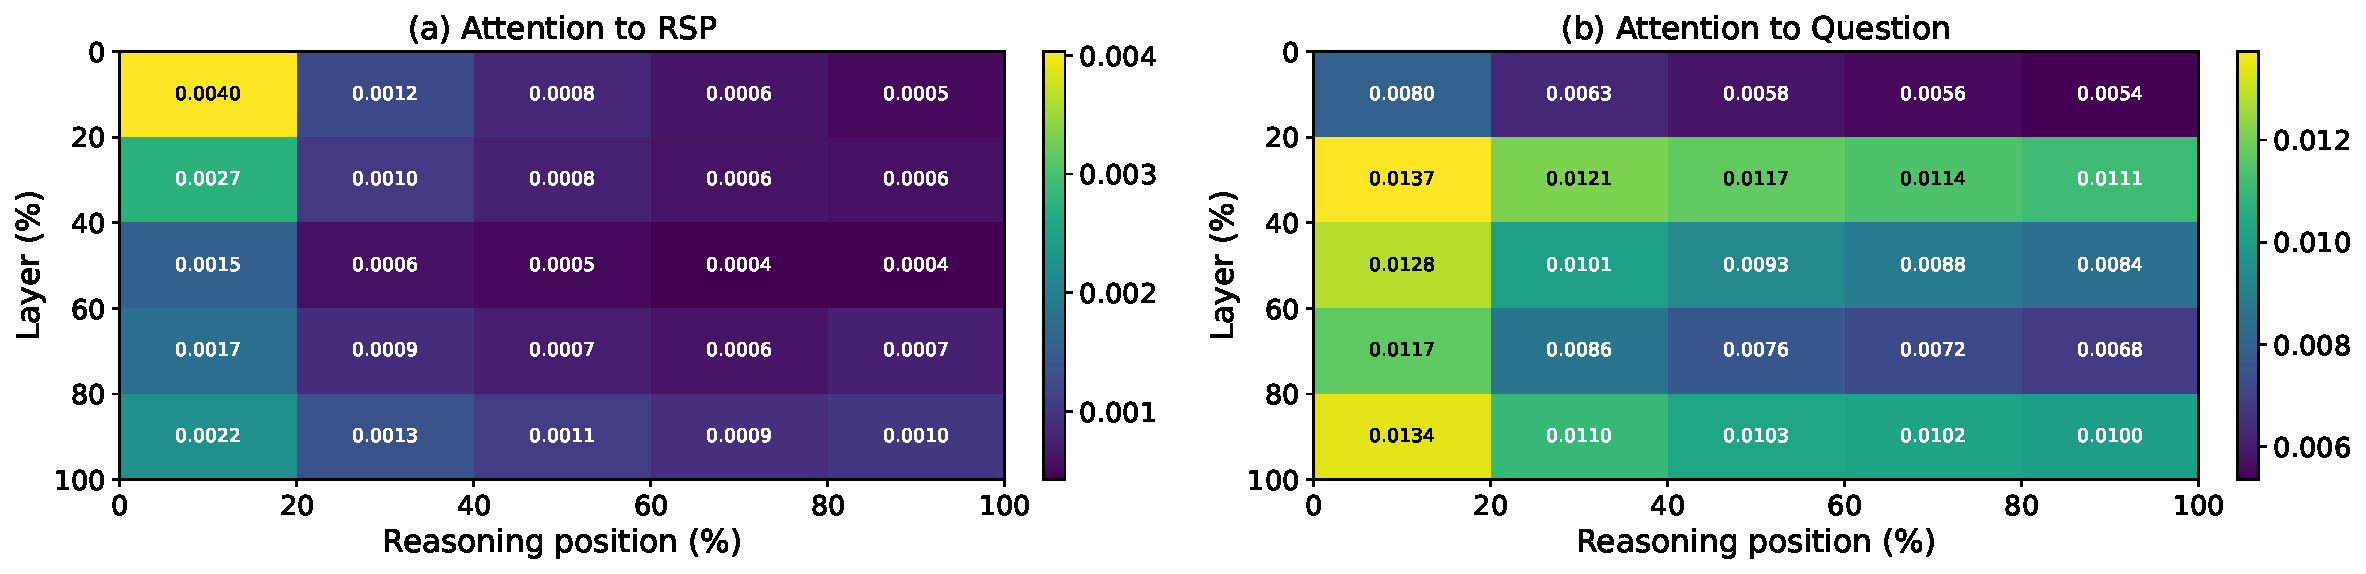
\includegraphics[width=0.9\textwidth]{img/attention/heatmap_qwen7b_suffix.pdf}
  \caption{Per-token attention mass on Qwen2.5-Math-7B (suffix, 500 MATH-500 problems, each with an independently sampled RSP). (a) RSP-token attention decreases along the reasoning-position axis, consistent with the KV cache-growth bound of Theorem~\ref{thm:decay}. The additional decrease along the layer axis is a separate empirical phenomenon suggesting that deeper layers sharpen the real-vs-random logit gap; it does not follow from Theorem~\ref{thm:decay} alone. (b) Question-token attention remains comparatively uniform. The reported quantity is the per-token mass of Appendix~\ref{app:attention_mass}, equal to $w_{r,i}^{(\ell)}/L$ averaged over heads and samples.}
  \label{fig:attention_mass}
\end{figure}

Lifting this single-shot branching to task accuracy via independent re-sampling across rollouts (\S\ref{sec:rsp_definition}) requires two assumptions: (M1) one execution reaches a correct trajectory with marginal probability $p_{\min}(x)>0$, and (M2) the $N$ executions are mutually independent. Under both, a standard ensemble argument yields $\Pr(\mathrm{Pass@}N \text{ on } x) \ge 1 - (1-p_{\min}(x))^N$ (Appendix~\ref{app:passN_ensemble}). \S\ref{sec:improve} showed that isotropy and full support together make single-shot branching reachable; \emph{independent resampling} now lifts those single-shot branches into an $N$-fold cumulative gain. Sharing one RSP across samples breaks (M2) and removes the accumulation, so independence is the key, exactly the signature documented empirically in \S\ref{sec:diversity}.
